
In the following, let $G$ be a compact group and $V,W$ be finite dimensional vector spaces. For the definitions we follow the textbook by \textcite{woit2016}.

\begin{definition}[Representation]
  A \emph{representation} of a compact group $G$ over a vector space $V$ is a group homomorphism
  \[
    \rho : G \to \GL V, \quad \rho(g)\rho(h) = \rho(g \cdot h), \quad \rho(e) = id_V
  \]
  The \emph{representation space} is the tuple $(\rho, V)$ but usually we shorten this to just $V$.
\end{definition}

\noindent
Equivalently we can state the definition of a representation of $G$ as imposed by its action on $V$, given as a map
  \begin{equation}
    \alpha : G \times V \to V, \quad (g,v) \mapsto g \cdot v
  \end{equation}
such that this is linear, todo. I think we get the equality to the hom def if we set $g \cdot v = \rho(g)v$

\begin{definition}[Intertwiner]
  A linear map $A : V \to W$ is an \emph{intertwiner}, if under representations $\rho_V : G \to \GL V$ and $\rho_W : G \to \GL W$ it holds that
  \[
    A \circ \rho_V(g) = \rho_W (g) \circ A \quad \forall g \in G.
  \]
  Denote the space of all intertwiners as $\Hom_G(V,W)$.
\end{definition}

\begin{definition}[Unitary representation]
  If our vector space $V$ is equipped  with a (Hermitian?) inner product 
\end{definition}

\begin{definition}[Irreducible representation (Woit 16)]
  A representation $\rho$ is an \emph{irrep} if there are no $W \subset V$ such that $(\rho_{\vert W}, W)$ is a representation. 
\end{definition}

\begin{definition}[Tensor product representation]
  Given reps $(\rho_V, V)$ and $(\rho_W, W)$, the \emph{tensor product representation} $(\rho_{V\otimes W}, V \otimes W)$ is defined by its action on the elements
  \[
    \rho_{V \otimes W}(g) (v \otimes w) = \rho_V(g) v \otimes \rho_W(g) w
  \]
\end{definition}

\begin{definition}[Direct sum representation]
  As above, the \emph{direct sum representation} $(\rho_{V \oplus W}, V \oplus W)$ 
  \[
    \rho_{V \oplus W}(g) = \begin{pmatrix}
      \rho_V(g) &   \\
       &  \rho_W(g) \\
    \end{pmatrix}
  \]
\end{definition}

\begin{definition}[Isotypic / Semisimple decomposition]
  Each semisimple representation $V$ decomposes as
  \[
    V \cong \bigoplus_{i \in I} V^{\oplus n_i}
  \]
  by grouping isomorphic simples. Is $n_i$ unique?
\end{definition}

During a theorem by Maschke \cite{}, the representations of any compact $G$ are semisimple. 
%Therefore, for any representations $V$ and $W$ it holds that
%\[
%  V \otimes W \cong \bigoplus_{c \in I} R_c^{\oplus m_c} 
%\]
%where $m_c$ is determined uniquely (why intuitively?) in dependece on the decompositions of $V$ and $W$:
%\[
%  V \otimes 
%\]

Therefore, it must hold for any irreps $R_a,R_b$ of $G$ that their tensor product is completely reducible with the decomposition
\[
  R_a \otimes R_b 
  \cong
  \bigoplus_{c \in I} R_c^{\oplus N_{ab}^c},
\]
with $N_{ab}^c$ called \emph{fusion-multiplicities}. If
\[
  N_{ab}^c \leq 1 \quad \forall a,b,c 
\]
the decomposition is said to be \emph{multiplicity-free}.

Note as well that the appearance of the \emph{direct sum} here (as discussed in \cref{cat:eq:fusionprop}) is fully characterized (carefull how i phrase this) by its injection and projection maps, for which we provide a graphical calculus.
\[
  \iota^{ab}_{c,\mu} : R_c \to R_a \otimes R_b \quad \text{ and } \quad \pi^{c,\mu}_{ab} : R_a \otimes R_b \to R_c \quad \text{ for } \mu \in 1,\ldots,N_{ab}^c  
\]
\begin{equation}
\begin{tikzpicture}[
    baseline=(current bounding box.center),
    scale=1.0,
    string arrow/.style={
        postaction={decorate},
        decoration={
            markings,
            mark=at position 0.55 with {\arrow[scale=1.0]{Stealth}}
        }
    }
]
\begin{scope}[xshift=-1cm]

\coordinate (a) at (0,0.6);
\coordinate (b) at (1.2,0.6);
\coordinate (v) at (0.6,1.2);
\coordinate (c) at (0.6,2);

\draw[string arrow] (c) -- (v);
\draw[string arrow] (v) -- (a);
\draw[string arrow] (v) -- (b);

\node[below] at (a) {$R_a$};
\node[below] at (b) {$R_b$};
\node[above] at (c) {$R_c$};

\node[right=1pt] at (v) {$\mu$};

\end{scope}

\begin{scope}[xshift=4cm]

\coordinate (a) at (0,2);
\coordinate (b) at (1.2,2);
\coordinate (v) at (0.6,1.2);
\coordinate (c) at (0.6,0.4);

\draw[string arrow] (a) -- (v);
\draw[string arrow] (b) -- (v);
\draw[string arrow] (v) -- (c);

\node[above] at (a) {$R_a$};
\node[above] at (b) {$R_b$};
\node[below] at (c) {$R_c$};

\node[right=1pt] at (v) {$\mu$};

\end{scope}
\end{tikzpicture}
\end{equation}


These maps are more commonly known as \emph{clebsch-gordan coefficients}.
%\[
%  \ket{a,i;b,j \vert C,c}
%\]

\begin{example}[Clebsch-Gordan series]
  Let $G = \SU{2}$ and let $V_i$ and $V_j$ be two spin irreps of charge $i$ and $j$. These combine to
  \begin{equation}
    (\pi_{V_i \otimes V_{j}}, V_i \otimes V_j) = \bigoplus_{k \in \left\vert i - j \right\vert}^{i + j} (\pi_{V_k}, V_k) \label{sym:eq:cgseries}
  \end{equation}
\end{example}



\subsection{Symmetric Tensors}

%Here we want to define tensors that are invariant under a symmetry $G$ (a compact group). We say that a tensor $T \in ()

Let $G$ be a compact group. Consider a tensor $T$ living in the tensor product space of its legs:
\[
  T \in V_1 \otimes \cdots \otimes V_n \otimes W_m^\ast \otimes \cdots \otimes W_1^\ast
\]

Let $\rho_i : G \to \GL{V_i}$ be the linear representation of $G$ on each vector space $V_i$, and let $\sigma_j^\ast : G \to \text{GL}(W_j^\ast)$ be the dual representation on $W_j^\ast$. 

The total action of the group $G$ on the entire tensor product space is given by
\begin{gather*}
  \Pi: G \to \text{GL}\left(\bigotimes_i V_i \otimes \bigotimes_j W_j^\ast\right) \\
  \Pi(g) = \rho_1(g) \otimes \cdots \otimes \rho_n(g) \otimes \sigma_m^\ast(g) \otimes \cdots \otimes \sigma_1^\ast(g)
\end{gather*}


A tensor $T$ is defined to be a \textbf{symmetric tensor} (or $G$-invariant tensor) if it is invariant under simultaneous action on all legs for all $g \in G$ \cite{singhTensorNetworkDecompositions2010a}:
\[
  \Pi(g) T = T \quad \forall g \in G
\]

Recall that by the isomorphism $\Hom(V,W) \cong W \otimes V^\ast$ as
\[
  w \otimes f \mapsto (v \mapsto f(v)w).
\]
We can push the product representation through this isomorphism as
\[
  \pi(g)(w \otimes f) = \rho_W(g)w \otimes \rho_{V^\ast}(g)f = \rho_W(g)w \otimes (\rho_V(g)^{-1})^T  f = \rho_W(g)w \otimes f(\rho_V(g)^{-1} )
\]
\[
  \cong v \mapsto f(\rho_V(g)^{-1}v ) \rho_W(g)w
\]

By interpreting $T$ as a map
\[
  T : W_1 \otimes \cdots \otimes W_m \to V_1 \otimes \cdots \otimes V_n
\]
it follows directly from the definition of global invariance that the tensor must commute with the group action and we get the following definition of a symmetric tensor:

\begin{definition}[symmetric tensor]
  \label{def:symmetricTensor}
  A \emph{symmetric tensor} is an intertwiner of the representations of the group $G$:
  \[
    \bigotimes_{j=1}^m \sigma_j(g) \circ T = T \circ  \bigotimes_{i=1}^n \rho_i(g) \quad \forall g \in G,
  \]
  which we denote by
  \[
    T \in Hom_G(W,V).
  \]
\end{definition}

\[
\begin{array}{c}
  \begin{tikzpicture}[
    baseline=(current bounding box.center),
    leg2/.style={
      line width=1.1pt,
      postaction={
        decorate,
        decoration={
          markings,
          mark=at position 0.7 with {\arrow{Stealth[scale=1.0, fill=black]}}
        }
      }
    },
    leg/.style={
        postaction={decorate},
        decoration={
            markings,
            mark=at position 0.55 with {\arrow[scale=1.0]{Stealth}}
        }
    },
    tensor/.style={
      draw=black,
      fill=white,
      line width=1.1pt,
      minimum size=18pt,
      inner sep=2pt,
      rectangle
    }
  ]
    

  \begin{scope}
    \node[tensor] (T1) at (0,0) {\scriptsize $T$};
    \draw[leg] (-1,0) node[left, yshift=2pt] {\tiny $A$} -- (T1.west) node[midway, above=2pt] {\scriptsize $U^\dagger$}; 
    \draw[leg] (T1.north) -- (0,1) node[above] {\tiny $B$} node[midway, right=2pt] {\scriptsize $U$};        
    \draw[leg] (T1.south) -- (0,-1) node[below] {\tiny $D$} node[midway, right=2pt] {\scriptsize $U$};        
    \draw[leg] (T1.east) -- (1,0) node[right, yshift=2pt] {\tiny $C$} node[midway, above=2pt] {\scriptsize $U$};        
  \end{scope}

  \node at (1.5,0) {$=$};

  \begin{scope}[xshift=3.0cm]
    \node[tensor] (T2) at (0,0) {\scriptsize $T$};
    \draw[leg] (-1,0) node[left, yshift=2pt] {\tiny $A$} -- (T2.west);       
    \draw[leg] (T2.north) -- (0,1) node[above] {\tiny $B$};       
    \draw[leg] (T2.south) -- (0,-1) node[below] {\tiny $D$};      
    \draw[leg] (T2.east) -- (1,0) node[right, yshift=2pt] {\tiny $C$};        
  \end{scope}

  \node at (4.8,0) {$\Longleftrightarrow$};


  \begin{scope}[xshift=6.8cm]
    \node[tensor] (T3) at (0,0) {\scriptsize $T$};
    \draw[leg] (-1,0) node[left, yshift=2pt] {\tiny $A$} -- (T3.west) node[midway, above=2pt] {\scriptsize $U^\dagger$}; 
    \draw[leg] (T3.north) -- (0,1) node[above] {\tiny $B$};
    \draw[leg] (T3.south) -- (0,-1) node[below] {\tiny $D$};
    \draw[leg] (T3.east) -- (1,0) node[right, yshift=2pt] {\tiny $C$};
  \end{scope}

  \node at (8.3,0) {$=$};

  \begin{scope}[xshift=10.1cm]
    \node[tensor] (T4) at (0,0) {\scriptsize $T$};
    \draw[leg] (-1,0) node[left, yshift=2pt] {\tiny $A$} -- (T4.west);                  
    \draw[leg] (T4.north) -- (0,1) node[above] {\tiny $B$} node[midway, right=2pt] {\scriptsize $U$};        
    \draw[leg] (T4.south) -- (0,-1) node[below] {\tiny $D$} node[midway, right=2pt] {\scriptsize $U$};        
    \draw[leg] (T4.east) -- (1,0) node[right, yshift=2pt] {\tiny $C$} node[midway, above=2pt] {\scriptsize $U$};        
  \end{scope}
  \end{tikzpicture}
  
  \\[2.0em] 

  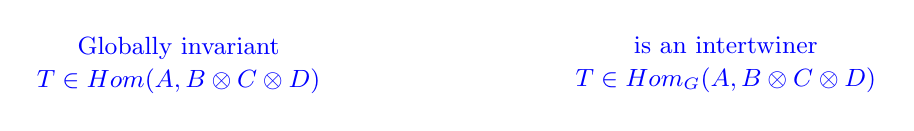
\begin{tikzpicture}[baseline=(current bounding box.center)]
    \node[anchor=north, align=center, text=blue] at (1.5,0) {
      \small Globally invariant \\
      \small $T \in \operatorname{Hom}(A, B \otimes C \otimes D)$
    };
    
    \node[anchor=north, align=center, text=blue] at (8.45,0) {
      \small is an intertwiner \\
      \small $T \in \operatorname{Hom}_G(A, B \otimes C \otimes D)$
    };
  \end{tikzpicture}
\end{array}
\]

\begin{corollary}[Networks of symmetric tensors are symmetric]
  Since a tensor network is built by composition and application of the $(co)ev$ maps, both of which are intertwiners, the full network is also an intertwiner. Important there is that this entire discussion is only about FdVect or FdHilb for now, but i think the same applies to any braided category.    
\end{corollary}

\subsection{Review of Symmetric Tensor Networks.}

The motivation for constructing symmetric tensor networks is as follows: Assume we have a (unitary) representation of a group $G$ denoted $U(g)$.  Furthermore assume we have a hamiltonian that commutes with $[U(g)^{\otimes L}, H] = 0$. If the ground state is unique, we can obtain 
\[
  U(g)^{\otimes L} H \ket{\psi_0} = H (U(g)^{\otimes L}) \ket{\psi_0} = E_0 U(g)^{\otimes L} \ket{\psi_0}
\]
and thus $U(g)\ket{\psi_{0} }$ is a ground state as well. By uniqueness
\[
  U(g) \ket{\psi_0} = e^{i\theta(g)} \ket{\psi_0}
\]

\begin{figure}[h]
  \centering
  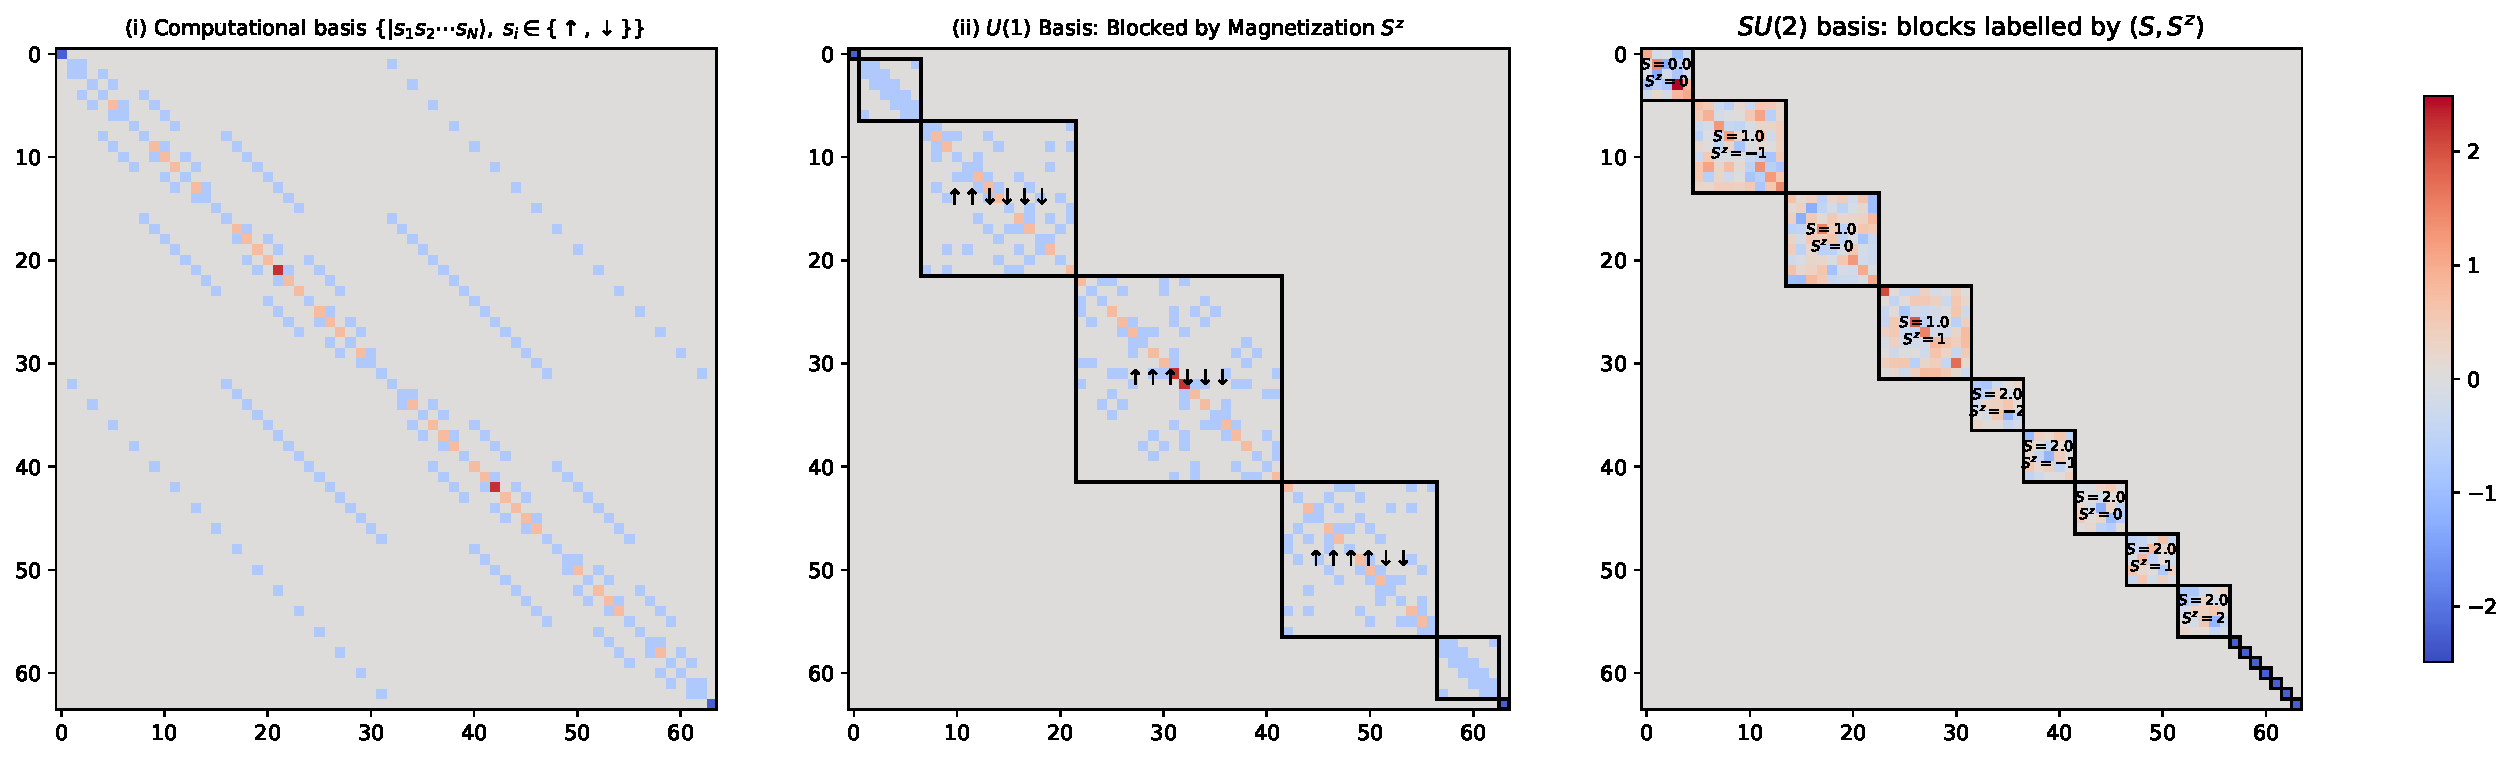
\includegraphics[width=\textwidth]{../experiments/plots/su2_block_structure.pdf}
  \caption{Three different presentations of the XXZ Hamiltonian. (i): In the default computational basis of spin vectors. (ii) In a reordering of the computational basis into equal spin up (down) classes, i.e. no spin up, one spin up etc..., here $U$ is simply a permutation matrix. (iii) After changing the basis into the $(S^2,S_Z)$ basis.}
  \label{fig:diagonal_hamiltonians}
\end{figure}

\begin{definition}[XXZ-Hamiltonian]
  \label{def:xxzHamiltonian}
  The XXZ Hamiltonian on $N$ sites is
  \begin{equation}
    H 
    = 
    J \cdot 
    \sum_{i = 1}^{N}
      (\sigma_i^x \sigma_{i+1}^x + \sigma_i^y \sigma_{i+1}^y + \Delta \sigma_i^z \sigma_i^z  ).
  \end{equation}
\end{definition}

As given in \cref{def:xxzHamiltonian}, this acts on the \emph{spin basis} made of states $\ket{s_1 s_2 \ldots s_n}$ where $s_i \in \{\uparrow, \downarrow\}$.

We can plot $H$ and realize the sparsity structure thereof. Furthermore, a suitable rearrangement induces a block structure \cref{fig:diagonal_hamiltonians}.

Now, we can realize about this hamiltonian is that there is a symmetry with the representations of $\U 1$. Lets review this shortly. A representation of $U(1)$ is a group homomorphism
\[
  \rho : \U 1 \to \GL V n , \quad \rho(e^{i\theta_1}) \rho(e^{i\theta_2}) = \rho(e^{i(\theta_1 + \theta_2)}). 
\]

The XXZ model lives in the Hilbert Space $\mathcal{\MakeUppercase{H}} = (\C^2)^{\otimes n}$ and the relevant representation is generated by the total magnetization operator
\[
  S^z_{\mathrm{tot}}
  =
  \frac12 \sum_{i = 1}^{N} \sigma_i^z
\]
The group action is given by
\[
  U(\theta)
  =
  e^{-i\theta S^z_{\mathrm{tot}}}.
\]

We now claim that $H$ is invariant under $U(\theta)$.
\[
  U(\theta) H U(\theta)^\dagger = H,
  \qquad \forall \theta \in \mathbb R.
\]
Equivalently,
\[
  [H,S^z_{\mathrm{tot}}]=0.
\]

Recall that when two operators commute, we can \emph{simultaneously diagonalize} them \cite[Theorem~1.3.12]{Horn_Johnson_2012}.

\begin{align*}
  [H, S^z_{\mathrm{tot}}] = \sum_{i}^{N} [\sigma_i^x \sigma_{i+1}^x + \sigma_i^y \sigma_{i+1}^y + \Delta \sigma_i^z \sigma_i^z, \sum_{j = 1}^{N} \sigma_j^z ] 
\end{align*}
and since operators on different sites commute, only $j = i$ and $j = i+1$ contribute. So we ought to write
\[
  \sum_{i}^{N} [\sigma_i^x \sigma_{i+1}^x + \sigma_i^y \sigma_{i+1}^y + \Delta \sigma_i^z \sigma_i^z, \sigma_i^z + \sigma_{i+1}^z  ] 
\]
and now using the identity $[AB,C] = A[B,C] + [A,C]B$:
\[
  [\sigma_i^x \sigma_{i+1}^x, \sigma_i^z + \sigma_{i+1}^z  ] = -2i(\sigma_i^y \sigma_{i+1}^x + \sigma_i^x \sigma_{i+1}^y  ) 
\]
\[
  [\sigma_i^y \sigma_{i+1}^y, \sigma_i^z + \sigma_{i+1}^z  ] = 2i(\sigma_i^x \sigma_{i+1}^{y} + \sigma_i^y \sigma_{i+1}^x  )
\]
which cancel out. Furtermore, the $z$ spins commute as well. Thus the whole sum is $0$ and we are done.

In the $\SU 2$ case, we have the generators
\[
  S_{tot}^\alpha = \frac{1}{2} \sum_{i = 1}^{N} \sigma_i^\alpha, \quad \alpha \in \{x,y,z\} 
\]

The representation here is  $U(R) = e^{i\theta n \cdot S_{tot} }$ and the Hamiltonian is invariant under
\[
  U(R) H U(R)^\dagger = H, \quad R \in \SU 2
\]

Since
\[
  [S_{tot}^x, S_{tot}^y ] = i S_{tot}^z 
\]
we need a new operator for the simulatenous diagonalization
\[
  S_{tot} = \sum_{a \in \{x,y,z\}}^{} (S_{tot}^{a})^2
\]
and we need to verify this is indeed the correct operator TODO.

The eigenvalues of $S_{tot}^2$ are  $S(S + 1)$ where  $S$ are the half integers.

Again, we can eithe solve htis by diagonalizing all 3 operators?

Or we can do the representation theoritical approach. Let $V_j$ denote the spin-$j$ irrep of $\SU 2$. We have that $\C^2 \cong V_{\frac{1}{2}}$ and by \cref{sym:eq:cqseries} that
\[
  (\mathbb{C}^2)^{\otimes6} \cong V_{\frac{1}{2}}^{\otimes 6} \cong 5 V_0 \oplus 9V_1 \oplus 5V_2 \oplus V_3 \cong \C^5 \otimes V_{\frac{1}{2}} \oplus \C^9 \otimes V_0 \oplus \C^5 \otimes V_2 \oplus V_3
\]

Now our operator is a morphism in $End(V_{\frac{1}{2}}^{\otimes 6})$ and thus by Schurs lemma\footnote{These are related by a permutation matrix. Proof? Is this the X from \cite{devosTensorKitjlJuliaPackage2025}? }
\begin{equation}\label{sym:eq:blockdiag}
  H \in \bigoplus_{S \in 0,1,2,3} Mat_{m_S \times m_S} \otimes I_{2S+1} (\mathbb{C}) \cong \bigoplus_{S \in 0,1,2,3} I_{2S+1} \otimes Mat_{m_S \times m_S}(\mathbb{C}) 
\end{equation}

So we expect 20 blocks? 
$5$ have dimension $1$, $9$ have dimension $3$, $5$ have dimension $5$ and $1$ has $7$.

To get an interpretation of the matrix coefficients in $\eqref{sym:eq:cgseries}$, consider a tiny Hamiltonian on $N = 2$ spins
\[
  H = \frac{1}{2} (\sigma_1^x \sigma_2^x + \sigma_1^y \sigma_2^y + \sigma_1^z \sigma_2^z)
  = S_1 \cdot S_2
\]

This acts on the space $V_{\frac{1}{2}} \otimes V_{\frac{1}{2}}$ and thus on the basis $\{\ket{\uparrow},\ket{\downarrow}\}^{\otimes 2}$ This has two distinct fusion outcomes, $V_0$ and $V_1$. The basis on the rhs is given by $\ket{1,1},\ket{1,0},\ket{1,-1}.\ket{0,0}$, and we want to reformulate $S_1 \cdot S_2$ in the total spin basis. Lets unfold this definition by 
\[
  S^2 = S_1^2 + S_2^2 + 2(S_1 \cdot S_2) \implies S_1 \cdot S_2 = \frac{1}{2}(S^2 - S_1^2 - S_2^2).
\]
Since $S_i^2 = s(s+1)$ is fixed for $s = \frac{1}{2}$ here, we ought to write
\[
  H = \frac{J}{2}(S^2 - 3/2)
\]
and this again splits into the sectors for $S = 0$
\[
  c_0 = \frac{J}{2}(0 - 3/2) = -\frac{3}{4}J
\]
and for $S = 1$ 
\[
  c_1 = \frac{J}{2}(2 - 3/2) = \frac{1}{4}J
\]
which are exactly the two degrees of freedom we get by the direct sum. So we expect our operator to look like
\[
  \begin{pmatrix}
    c_0 &  0 \\
    0 &  \id_3 \otimes c_1 \\
  \end{pmatrix}.
\]

By direct isomorphism, we can write this as
\begin{equation}\label{sym:eq:S1S2}
\begin{tikzpicture}[
    baseline=(current bounding box.center),
    scale=1.0,
    string arrow/.style={
        postaction={decorate},
        decoration={
            markings,
            mark=at position 0.55 with {\arrow[scale=1.0]{Stealth}}
        }
    }
  ]
  
  \node at (0.8,2.0) {$\displaystyle -J\frac{3}{4}\,\otimes$};
  \coordinate (bot_a) at (1.1, 1.0);
  \coordinate (bot_b) at (2.1, 1.0);
  
  \node at (1.6, 0.7) {$\underbrace{\quad\quad}_{\text{dim} 1}$};


  \coordinate (mid_bot) at (1.6, 1.6);
  \coordinate (mid_top) at (1.6, 2.4);
  
  \coordinate (top_a) at (1.1, 3.0);
  \coordinate (top_b) at (2.1, 3.0);

  \draw[string arrow] (bot_a) -- (mid_bot);
  \draw[string arrow] (bot_b) -- (mid_bot);
  
  \draw[string arrow] (mid_bot) -- (mid_top) node[right, pos=0.5] {$0$};
  
  \draw[string arrow] (mid_top) -- (top_a) node[above] {$\frac{1}{2}$};
  \draw[string arrow] (mid_top) -- (top_b) node[above] {$\frac{1}{2}$};
  
  \node at (2.5, 2.0) {$\oplus$};

\begin{scope}[shift={(2.2,0.0)}]
  \node at (1.0,2.0) {$\displaystyle\frac{J}{4}\,\otimes$};
  \coordinate (bot_a) at (1.1, 1.0);
  \coordinate (bot_b) at (2.1, 1.0);
  
  \node at (1.6, 0.7) {$\underbrace{\quad\quad}_{\text{dim} 3}$};

  \coordinate (mid_bot) at (1.6, 1.6);
  \coordinate (mid_top) at (1.6, 2.4);
  
  \coordinate (top_a) at (1.1, 3.0);
  \coordinate (top_b) at (2.1, 3.0);


  \draw[string arrow] (bot_a) -- (mid_bot);
  \draw[string arrow] (bot_b) -- (mid_bot);
  
  \draw[string arrow] (mid_bot) -- (mid_top) node[right, pos=0.5] {$1$};
  
  \draw[string arrow] (mid_top) -- (top_a) node[above] {$\frac{1}{2}$};
  \draw[string arrow] (mid_top) -- (top_b) node[above] {$\frac{1}{2}$};
\end{scope}

\end{tikzpicture}
\end{equation}



\begin{definition}[Matrix Product State]
  \label{def:MPS}
  A \emph{Matrix Product State} is a quantum state $\ket{\psi}$ with $n$ legs written as the contraction of $n$ trivalent tensors $\{A^{[i]}\}_{i \in [n]}$. Formally this reads
  \[
    \ket{\psi[A]}
    =
    \sum_{i_1,\ldots,i_n}
    \operatorname{Tr}\!\left(
    A^{[1]}_{i_1}
    A^{[2]}_{i_2}
    \cdots
    A^{[n]}_{i_n}
    \right)
    \ket{i_1i_2\cdots i_n},
  \]
  where $A^{[i]}_{i_{k}} \in \mathbb{C}^{D_i \times D_{i+1} }$. The elements of the collection $\{D_i\}_{i \in [n]}$ is referred to as the \emph{bond-dimensions}.
\end{definition}
Note that this is a state with closed boundaries. If we want open boundaries we have to replace the trace with appropriate end vectors (nice source?).

\begin{example}
  We can represent each product state $\ket{\varPsi} = \ket{\psi}^{\otimes n}$ as a MPS with bond dimension $1$.
\end{example}

\begin{theorem}[Fundamental Theorem of MPS]
  If two MPS states generated by $A$ and $B$ respectively.
  Figure out what we can do with this. 
  
  Proof \cite{ciracMatrixProductDensity2017},\cite{vercleyenMathematicalStructureTensor2018}, \cite{perez-garciaStringOrderSymmetries2008a}.
\end{theorem}